\documentclass[12pt,a4paper]{article}
\title{%
  Øving 5 \\
  \large IFYKJT1001 - Fysikk/Kjemi \\
  }
\author{Gunnar Myhre, BIELEKTRO}

\usepackage[utf8]{inputenc}
\usepackage[norsk]{babel}
\usepackage{amsmath}
\usepackage{siunitx}

\usepackage{graphicx}
\graphicspath{ {./images} }

\setlength\parindent{0pt}

\begin{document}
  \maketitle

  \section*{Oppgåve 1}
    \subsection*{a)}
    Kulas starthøgde er gitt som
    \begin{equation}
      h=Lsin(\theta)
    \end{equation}
    kulas potensielle energi i øverste posisjon er
    \begin{equation}
      U=mgh\rightarrow U = mgLsin(\theta)
    \end{equation}
    i botnen av skråplanet har kula ingen potensiell energi, og all energien
    er omgjort til kinetisk energi
    \begin{equation}
      U_1 = K_2
    \end{equation}
    den kinetiske energien på botnen er gitt som
    \begin{equation}
      K_2 = \frac{1}{2}mv^2
    \end{equation}
    setter saman likningene og finner farta i botnen av skråplanet
    \begin{equation}
      U_1 = K_2 \rightarrow mgLsin(\theta) = \frac{1}{2}mv^2 \rightarrow
      v = \sqrt{2gLsin(\theta)} = 3,67[m/s]
    \end{equation}
    finner den kinetiske energien på botnen av skråplanet
    \begin{equation}
      K_2 = \frac{1}{2}mv^2 = 18,87[J]
    \end{equation}

    \subsection*{b)}
    \subsubsection*{1)}
    Vi kan bruke den tidlause bevegelseslikninga for konstant akselerasjon for å finne
    farta til kulas massesentrum i botnen av skråplanet
    \begin{equation}
      v^2 = 2as \rightarrow v = \sqrt{2as} = 3,11 [m/s]
    \end{equation}
    ut ifrå denne farta kan vi finne vinkelfarta sidan kula ikkje glir eller spinner
    \begin{equation}
      \omega = \frac{v}{R} \rightarrow \omega = 207 [rad/s]
    \end{equation}

    \subsubsection*{2)}
    Vi veit at den kinetiske energien til kula i botnen av planet $K_2$ er lik
    den potensielle energien $U_1=mgLsin\theta$ på toppen av planet, som vi fant i oppgåve
    \textbf{a}. Finner formel for treghetsmoment for massiv kule i
    formelsamlinga $I = \frac{2}{5}MR^2$ og setter opp likninga
    \begin{equation}
      K_2 = \frac{1}{2}mV^2 + \frac{1}{2}I_{cm}\omega^2 \longrightarrow
      mgLsin(\theta) = \frac{1}{2}mV^2 + \frac{1}{2}\frac{2}{5}mR^2 \omega^2
    \end{equation}
    Sidan kula ikkje spinner eller glir er kontaktpunktet mellom kula og skrårampa
    i ro, då stemmer forholdet $V_{cm} = R\omega$. Setter inn for $V_{cm}$ og
    forenkler algebraisk
    \begin{equation}
      gLsin(\theta) = \frac{1}{2}R^2\omega^2 + \frac{1}{5}R^2\omega^2
    \end{equation}
    finner uttrykk for $\omega$
    \begin{equation}
      \omega = \sqrt{\frac{gLsin(\theta)}{\frac{1}{2}R^2+\frac{1}{5}R^2}} = 207 [rad/s]
    \end{equation}
    setter inn i $V = R\omega$ for å finne massesentrumets fart
    \begin{equation}
      V_{cm} = R\omega = 3,11 [m/s]
    \end{equation}
    dette stemmer overeins med svara frå oppgåve \textbf{b1}.

    \newpage
    
    \subsection*{c)}
    Definerer x-retning langs skråplanet.
    \begin{center}
      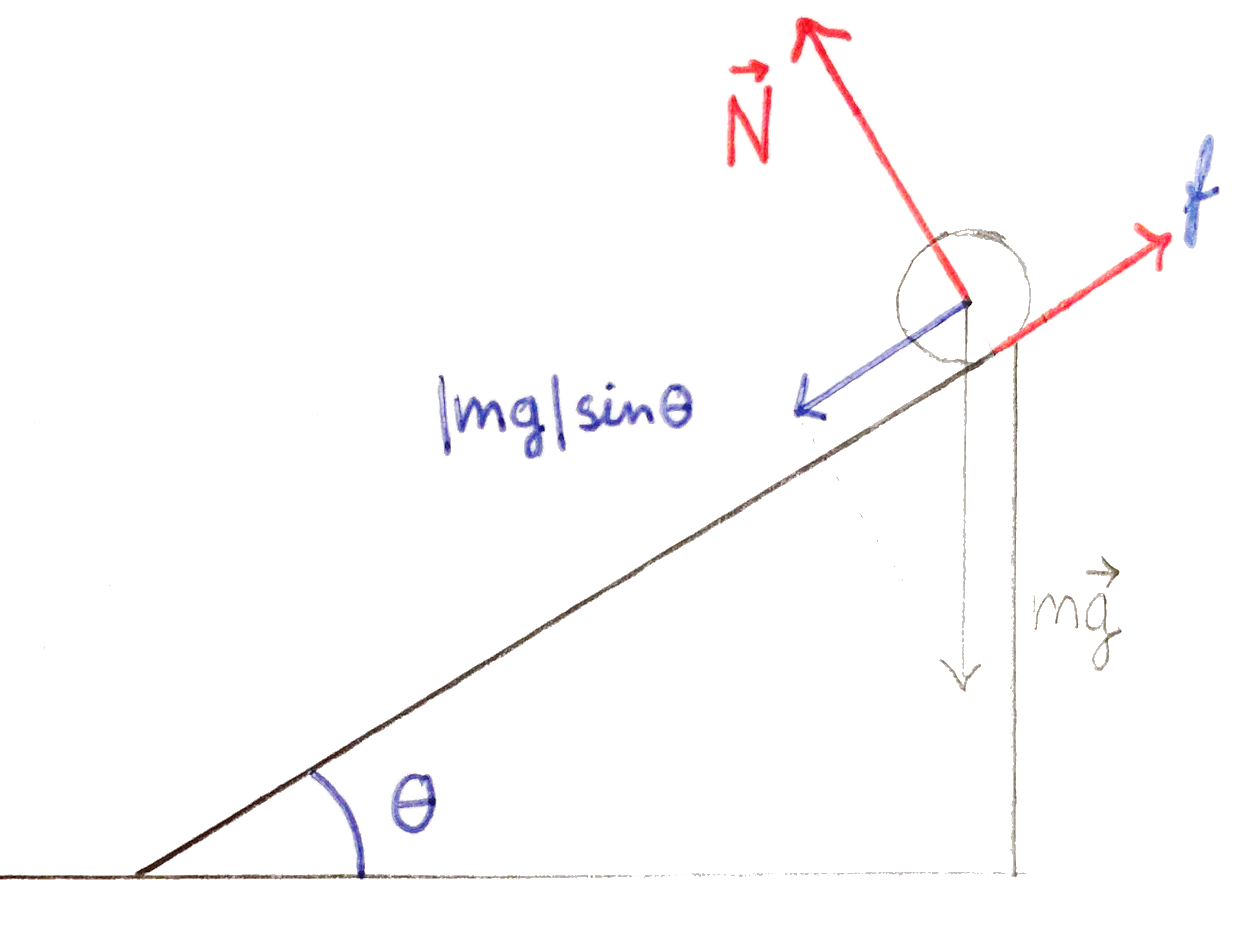
\includegraphics{05_1c}
    \end{center}
    Summen av kreftene i x-retning er gitt ved Newtons andre lov som massa
    gonger akselerasjonen i x-retning. Kreftene som verker i x-retning er den
    dekomponerte gravitasjonskrafta og friksjonskrafta.
    \begin{equation}
      \Sigma F_x = ma_{cm} \rightarrow mgsin(\theta) - f = ma_{cm} \rightarrow f=4,50[N]
    \end{equation}
    Alternativt kan vi finne $f$ ved Newtons andre lov for rotasjon.
    \begin{equation}
      \Sigma \tau = I\alpha \rightarrow fR = \frac{2}{5}mR^2\alpha \rightarrow f=4,50[N]
    \end{equation}

    \subsection*{d)}
    Veldig generelt kan vi seie at 
    \begin{equation}
      U_A = U_B + K_B
    \end{equation}
    Sidan $h_A > h_B$, og sidan den einaste krafta som verker på kula er gravitasjonen vil kula
    gå ei heil runde rundt loopen. Vidare kan vi bryte den kinetiske delen av energien opp i
    translasjon og rotasjon
    \begin{equation}
      U_A = U_B + \frac{1}{2}mv_{cm}^2 + \frac{1}{2}I_{cm}\omega^2
    \end{equation}
    Vi kan sette inn for treghetsmomentet $I=\frac{2}{5}mR^2$ og uttrykk for dei potensielle
    energiane, som gitt av kulas høgde over nullnivået
    \begin{equation}
      mgLsin\theta = mgy + \frac{1}{2}mv_{cm}^2 + \frac{1}{5}mR^2\omega^2
    \end{equation}
    der $y$ er høgda kula har over nullnivået. Sidan vi antar at kula ikkje
    glir eller spinner stemmer forholdet $V_{cm} = R\omega$. Vi ser også at
    modellen er uavhengig av massa til kula
    \begin{equation}
      gLsin\theta = gy + \frac{1}{2}v_{cm}^2 + \frac{1}{5}v_{cm}^2
    \end{equation}
    sidan det ikkje er definert noko spesifikt mål med å sette opp denne likninga velger
    eg å stoppe her.

  \section*{Oppgåve 2}
    \subsection*{a)}
    \begin{center}
      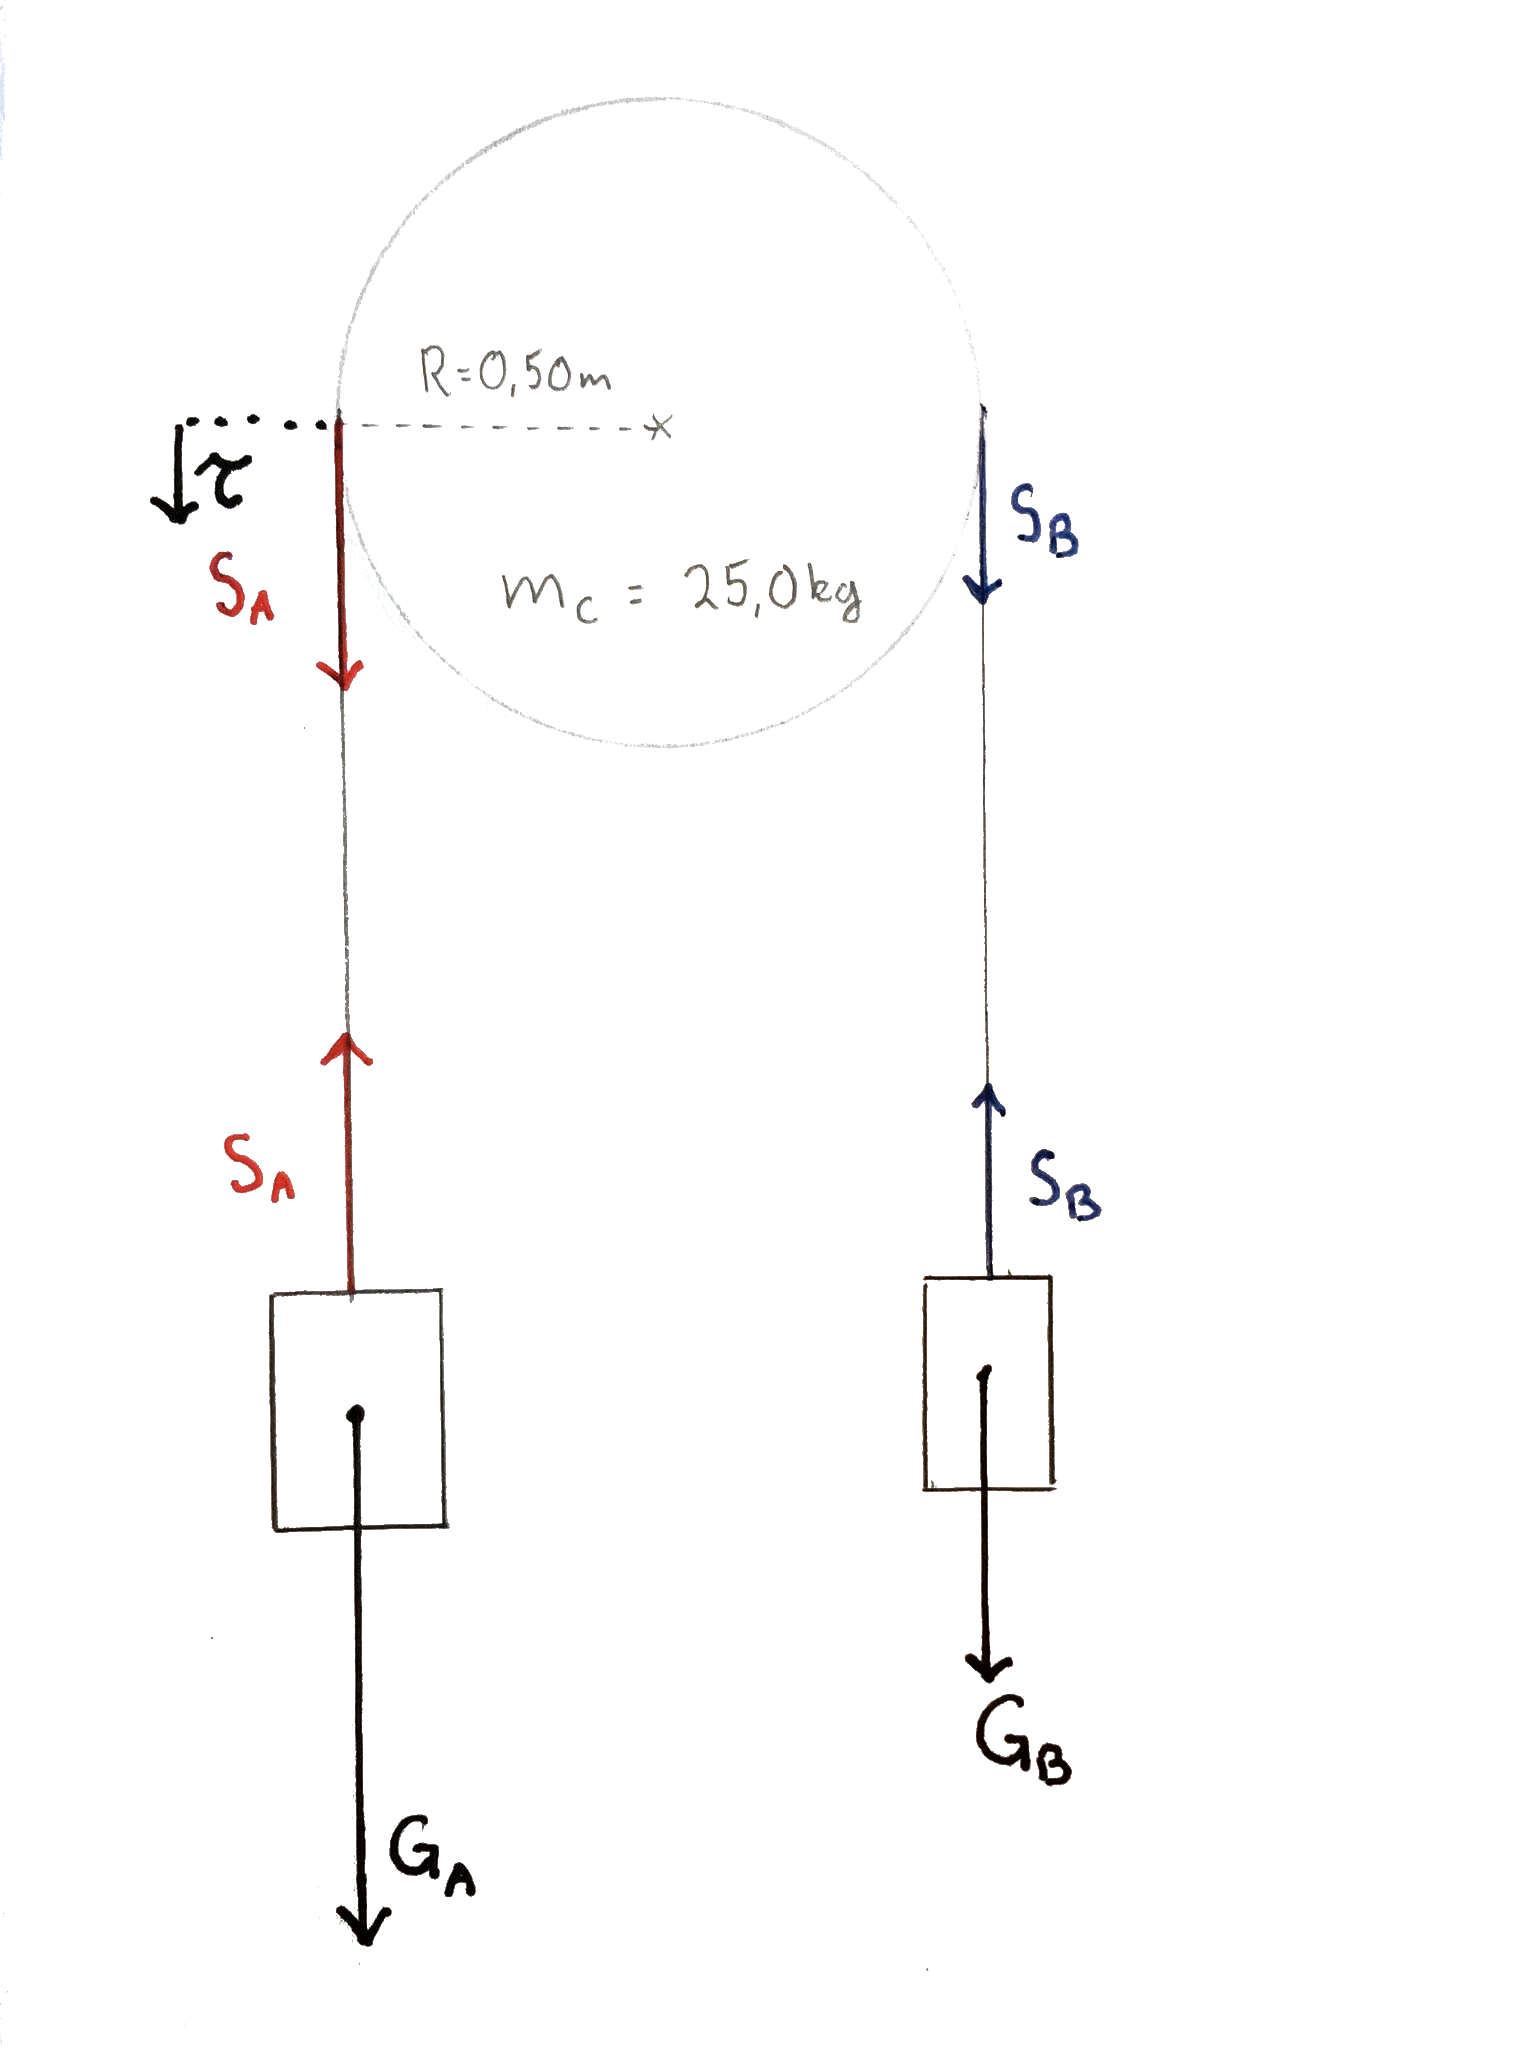
\includegraphics[scale=0.7]{05_2a}
    \end{center}

    \subsection*{b)}
    \begin{itemize}
      \item $G_A - S_A = m_Aa \rightarrow S_A = G_A - m_Aa$
      \item $S_B - G_B = m_Ba \rightarrow S_B = m_Ba + G_B$
      \item $(\Sigma \tau)_{ytre} = I\alpha \rightarrow (S_A - S_B)R = I\alpha$
    \end{itemize}
    Løyser likningssettet algebraisk
    \begin{equation}
      (G_A - m_Aa - m_Ba - G_B)R = I\alpha
    \end{equation}
    Vi kan beskrive treghetsmomentet til trinsa som ein massiv sylinder $I=\frac{1}{2}mR^2$.
    \begin{equation}
      (G_A - m_Aa - m_Ba - G_B)R = \frac{1}{2}m_cR^2\alpha
    \end{equation}
    vi veit at $\alpha = \frac{a}{R}$
    \begin{equation}
      (G_A - m_Aa - m_Ba - G_B) = \frac{1}{2}m_cR\frac{a}{R}
    \end{equation}
    gravitasjonskreftene er gitt som $G=mg$
    \begin{equation}
      (m_Ag - m_Aa - m_Ba - m_Bg) = \frac{1}{2}m_ca
    \end{equation}
    forenkler algebraisk for å finne uttrykk for akselerasjonen
    \begin{equation}
      a = \frac{(m_A - m_B)g}{\frac{1}{2}m_C + m_A + m_B} \rightarrow a = 2,00[m/s^2]
    \end{equation}

    \subsection*{c)}
    Vi kan finne numeriske størrelsar for snordraga
    \begin{itemize}
      \item $S_A = G_A-m_Aa \rightarrow S_A = 273 [N]$
      \item $S_B = m_Ba+G_B \rightarrow S_B = 248 [N]$
    \end{itemize}

    \subsection*{d)}
    Dei to snordraga $S_A$ og $S_B$ er ikkje eit kraftpar i dette tilfellet,
    sidan dei verker på trinsa og ikkje på kvarandre. Dette overholdast nettop
    av at tråden ligger over trinsa i eit tilfelle av statisk friksjon, som
    oppgitt i oppgåveteksten. I tilfellet det ikkje er nokon friksjon mellom
    tråden og trinsa vil $S_A$ og $S_B$ vere eit kraftpar og Newtons tredje lov
    til gjelde.

  \section*{Oppgåve 3}
    \begin{center}
      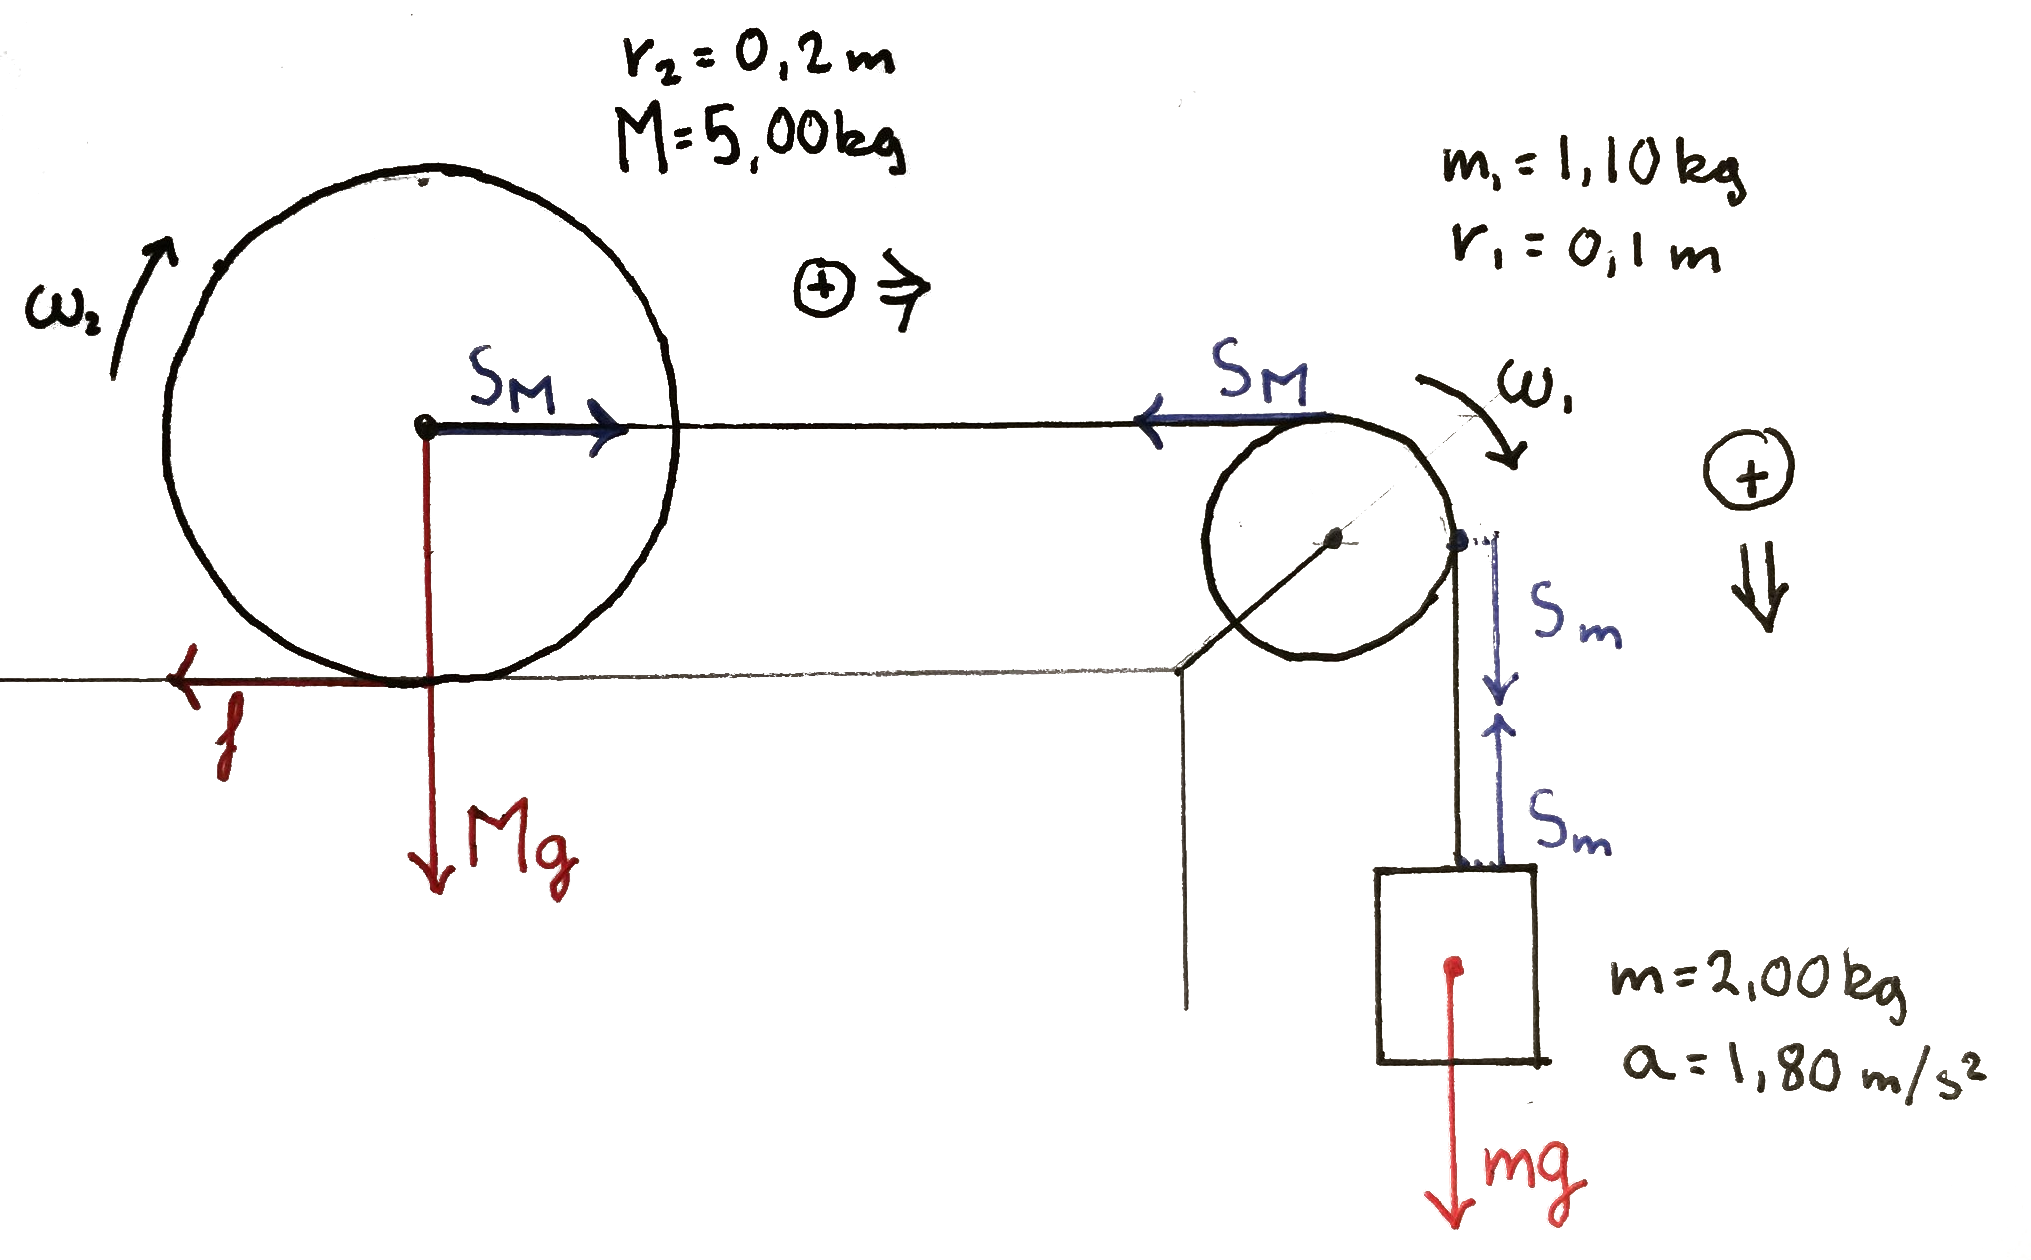
\includegraphics[scale=0.7]{05_3}
    \end{center}
    \subsection*{a)}
    Gravitasjonskrafta
    \begin{equation}
      mg = 2,00kg \cdot 9,81m/s^2 = 19,6 [N]
    \end{equation}
    og snordraget
    \begin{equation}
      S_m = G_m - ma = 16,0[N]
    \end{equation}

    \subsection*{b)}
    snordraget mot loddet
    \begin{equation}
      S_m = G_m - ma = 16,0[N]
    \end{equation}
    snordraget mot tønna kan vi finne ved Newtons andre lov for rotasjon
    \begin{equation}
      (\Sigma \tau)_{ytre} = I\alpha \rightarrow
      (S_m - S_M)r_1 = \frac{1}{2}m_1r_1^2\alpha
    \end{equation}
    vi veit at $\alpha = \frac{a}{r}$
    \begin{equation}
      S_m - S_M = \frac{1}{2}m_1r_1\frac{a}{r_1} \rightarrow S_M = S_m - \frac{1}{2}m_1a
      \rightarrow S_M = 15,0[N]
    \end{equation}

    \subsection*{c)}
    Vi har gravitasjonskrafta
    \begin{equation}
      Mg = 49,1[N]
    \end{equation}
    og snordraget mot trinsa
    \begin{equation}
      S_M = 15,0[N]
    \end{equation}
    og friksjonskrafta i kontaktpunktet mellom tønna og bakken, denne kan vi finne med
    Newtons andre lov
    \begin{equation}
      \Sigma F = ma \longrightarrow S_M - f = Ma \rightarrow f = S_M - Ma = 6,01[N]
    \end{equation}
    Treghetsmomentet til tønna kan vi finne nå som vi kjenner friksjonskrafta
    \begin{equation}
      \Sigma \tau = I \alpha_z \rightarrow f\cdot r_2 = I \frac{a}{r_2} \rightarrow
      I = \frac{fr_2^2}{a} \rightarrow I = 0,134[kgm^2]
    \end{equation}


  \subsection*{Oppgåve 4}
    Først er all energien potensiell, vi setter punktet $l$ som nullpunkt
    \begin{equation}
      U = mgl
    \end{equation}
    deretter, i punktet $l$, er all energien kinetisk. Denne er vi ikkje
    interesserte i nå. Etter punktet $l$ går energien igjen over i potensiell
    energi i strikken, dette medfører at hopparen bremser ned. Denne
    potensielle energien er gitt som $U=\frac{1}{2}kx^2$.
    Energibevaringslikninga ser slik ut
    \begin{equation}
      mgl = \frac{1}{2}kx^2
    \end{equation}
    som er alternativ \textbf{A}.



\end{document}
